\section{Measured Anti-Recomputation Gains}

The strongest measured results in this paper appear when the reused stage
actually owns meaningful wall-clock. Those gains are not one number. They are
regime-dependent, and the figure below is designed to make that obvious rather
than hide it.

\IfFileExists{generated/tables/headline_results.tex}{
\begin{table}[H]
\centering
\caption{Main speedup cells. Rows use different denominators; C-CEILING explains why they do not multiply.}
\label{tab:headline-results}
\scriptsize
\setlength{\tabcolsep}{2pt}
\renewcommand{\arraystretch}{\PaperTableStretch}
\begin{tabularx}{\linewidth}{@{}>{\raggedright\arraybackslash}p{0.12\linewidth} Y >{\raggedright\arraybackslash}p{0.15\linewidth} >{\raggedright\arraybackslash}p{0.10\linewidth} Y >{\raggedright\arraybackslash}p{0.12\linewidth}@{}}
\toprule
Regime & Setting & Speedup denominator & Gain & Validation / notes & Evidence \\
\midrule
After-ingest repair & Qwen adaptive repair breadth & cold/repaired follow-up & 14.90--35.92$\times$ & choice 0/93; correct 0/93; cold-all-query ratio 15.28--35.97$\times$ & repair breadth \\
After-ingest repair & Qwen fixed \(K=1\) repair breadth & cold/repaired follow-up & 9.48--20.37$\times$ & choice 0/93; correct 0/93; pathological follow-ups 0/62 & repair breadth \\
After-ingest raw & Qwen raw warm reuse, 16f & cold/cached follow-up & 91.1$\times$ & 0.807\,s median; $\Delta$acc +0.000 & aggregate-clean; unrepaired \\
After-ingest raw & Qwen raw warm reuse, 8f & cold/cached follow-up & 47.2$\times$ & 0.815\,s median; $\Delta$acc -0.048 & within criterion \\
First-pass & Gemma VideoMME 8f holdout & first-query E2E & 1.113$\times$ & $\Delta$acc +0.000 & aggregate-clean \\
First-pass & Gemma sparse vision, 32f short & first-query E2E & 1.316$\times$ & choice agreement 100\%; $\Delta$acc +0.000; dense parse 0; sparse parse 0 & \PaperStack{clean}{timed-skip} \\
First-pass & Gemma MVBench 8f holdout & first-query E2E & 1.407$\times$ & $\Delta$acc -0.033; timing-attribution caveat & advisory \\
First-pass & Qwen sparse vision, 16f \(kr_V=0.85\) & first-query E2E & 1.032$\times$ & $\Delta$acc -0.050; vision reduction 13.6\%; parse failures 0; agreement 81.7\% & format gate; low gain \\
\bottomrule
\end{tabularx}
\end{table}

}{
\draftnote{Run \texttt{make paper-sync} to generate the headline results table.}
}

\begin{figure}[H]
  \centering
  \IfFileExists{generated/figures/headline_results.pdf}{
    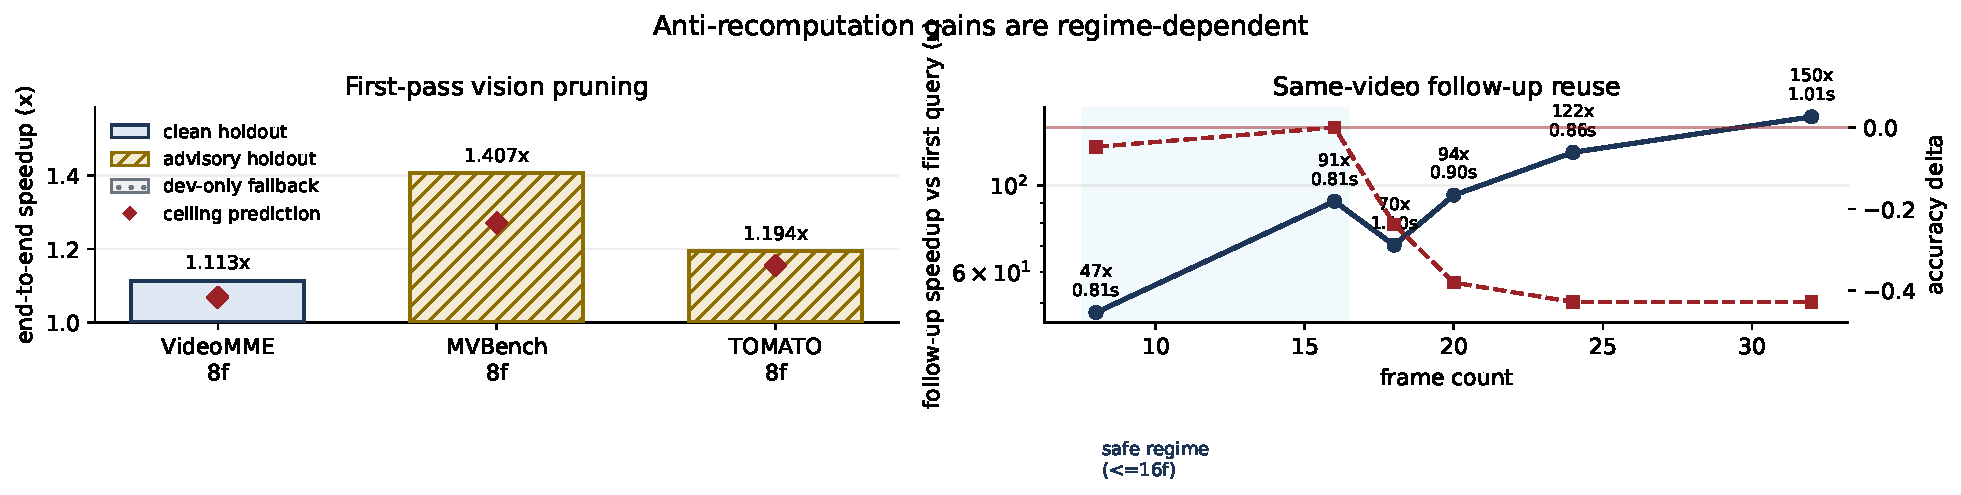
\includegraphics[width=\linewidth]{generated/figures/headline_results}
  }{
    \fbox{\parbox{0.9\linewidth}{Run \texttt{make paper-sync} to generate the headline results figure.}}
  }
  \caption{Headline anti-recomputation results by regime. Left: first-pass
  Gemma vision-pruning speedups with scatter-back ceiling predictions. Right:
  Qwen persistent-KV follow-up speedups versus frame count, with accuracy delta
  tracked separately. Hatched bars indicate advisory or dev-only status rather
  than clean holdout.}
  \label{fig:headline-results}
\end{figure}

\subsection{Orders Of Magnitude For Reuse, Modest Multipliers For Fresh Video}

The largest multipliers here belong to after-ingest reuse: 47.2$\times$ at 8
frames and 91.1$\times$ at 16 frames, both with sub-second follow-up latency.
That is not a contradiction with the smaller first-pass numbers. It is the
expected consequence of reusing an already-paid prefix instead of pruning only
one stage of a fresh-video pass.

\subsection{First-Pass Gains Are Real, But Share-Limited}

Fresh-video first-pass gains are smaller because they are share-limited. Gemma
vision-tower pruning still produces measured end-to-end gains before any
same-video caching trick enters the picture. VideoMME 8f is clean at
1.113$\times$ with zero aggregate accuracy delta. MVBench 8f is stronger still
at 1.407$\times$, with a small accuracy loss and an advisory thermal note
because the short decode window makes the old relative gate too strict for
scheduler-scale jitter. TOMATO 8f is advisory as well: the freshly pulled
upstream rerun reports 1.194$\times$ with a favorable-direction 19\,ms thermal
miss.

Their magnitude tracks the dense share owned by the vision tower. The same
pruning mechanism gives smaller gains on VideoMME than on MVBench because
VideoMME is less vision-dominated at this geometry. That is exactly what the
ceiling law predicts.

\subsection{After-Ingest Reuse Is The Big-Number Regime}

Persistent-KV answers a different question: once the first query on a video has
already paid the full prompt cost, how cheap can the next question become? On
Qwen2.5-VL-7B-4bit, the answer is already large enough to matter. At 8 frames,
follow-up latency drops to 815\,ms median with 47.2$\times$ speedup and
$-0.048$ aggregate accuracy delta. At 16 frames the speedup rises to
91.1$\times$ while the accuracy delta returns to 0. Within the current
$\leq$16f envelope, the result is both fast and empirically clean. Past that
point the curve keeps rising, but the fidelity boundary appears. That is a
useful result in its own right. The big numbers are tied to a concrete
after-ingest regime with a measurable safe envelope.

\subsection{The Story Is Stronger Because The Regimes Are Separate}

The measured first-pass gains and the after-ingest gains complement rather than
compete with each other. First-pass pruning says there is real work to skip on
fresh videos, but the ceiling is share-limited. Persistent-KV says that once a
video has already been ingested, the next question is a much larger reuse
opportunity. The Qwen routing section that follows explains why: temporal
placement of fresh compute decides whether the answer survives.

\begin{sectiontodo}{Lock the final promotion boundary for advisory cells}
The current figure and table are accurate, but the manuscript still needs a
final venue-facing decision on how aggressively to surface advisory rows in the
main text versus the appendix. VideoMME is clean. MVBench and TOMATO are
strong, but they should keep their caveats visible.

\textcolor{todoBorder}{Source pointers: \path{paper/priority.md},
\path{paper/claim-matrix.md},
\path{research/experiments/2026/2026-04-21-phase-1_51V-session3-findings.md},
\path{research/experiments/2026/2026-04-21-phase-1_51V-session4-findings.md},
\path{research/experiments/2026/2026-04-19-phase-1_55A-persistent-kv-findings.md},
\path{research/experiments/2026/artifacts/phase1_55A_*},
\path{codec-through/research/experiments/2026/2026-04-21-phase-1_51V-session5-findings.md}.}
\end{sectiontodo}
